% You should title the file with a .tex extension (hw1.tex, for example)
\documentclass[11pt]{article}

\usepackage{amsmath}
\usepackage{amssymb}
\usepackage{fancyhdr}
\usepackage{enumerate}
\usepackage{hyperref}


\usepackage{graphicx}
\graphicspath{ {images/} }

\oddsidemargin0cm
\topmargin-2cm     %I recommend adding these three lines to increase the 
\textwidth16.5cm   %amount of usable space on the page (and save trees)
\textheight23.5cm  

\newcommand{\question}[2] {\vspace{.25in} \hrule\vspace{0.5em}
\noindent{\bf #1: #2} \vspace{0.5em}
\hrule \vspace{.10in}}
\renewcommand{\part}[1] {\vspace{.10in} {\bf (#1)}}

\newcommand{\myname}{Bryce Summers, Brandon Lum}
\newcommand{\myandrew}{bwsummer, jiajunbl}
\newcommand{\bigO}{\mathcal{O}}

\setlength{\parindent}{0pt}
\setlength{\parskip}{5pt plus 1pt}
 
\pagestyle{fancyplain}
\lhead{\fancyplain{}{\textbf{Final Project Writeup}}} % Note the different brackets!
\rhead{\fancyplain{}{\myname\\ \myandrew}}
\chead{\fancyplain{}{15-418}}

\begin{document}

\medskip                        % Skip a "medium" amount of space
                                % (latex determines what medium is)
                                % Also try: \bigskip, \littleskip

\thispagestyle{plain}
\begin{center}                  % Center the following lines
{\Large Random Maze Generation: 15-418 Final Writeup} \\
\myname \\
\myandrew \\

\today \\
\end{center}


\question{Summary}

We implemented \textbf{lock-free Union find structures} to parallelize an inherently serial random maze construction algorithm and therebye \textbf{solve the random maze construction problem faster.}\\

Using lock-free Union find structures, we achieved a consistent speedup using \textbf{8-threads} of around \textbf{2x} for the \textbf{critical loop} of the maze construction algorithm \textbf{relative to} the performance of the \textbf{serial algorithm} utilizing a standard serial union find structure. This is sufficient for helping out a professional using a \textbf{standard commodity computer.}
\\

\begin{figure}[h]
\centering
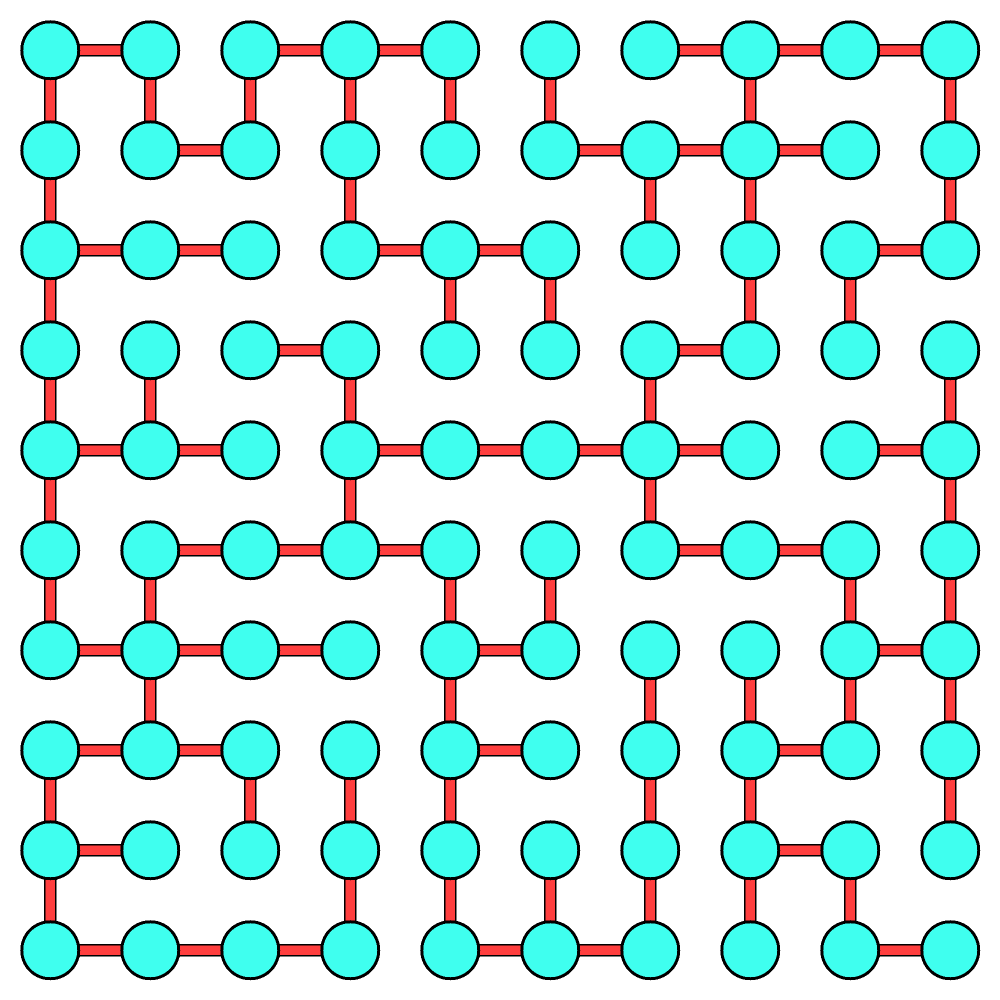
\includegraphics[width=0.5\textwidth]{Lattice2}
\caption{Example Generated Maze}
\label{fig:TitlePage}
\end{figure}

\href{https://github.com/Bryce-Summers/Randomized_Acyclic_Connected_Sub_Graphs}{Project Repository:}\\
\url{https://github.com/Bryce-Summers/Randomized_Acyclic_Connected_Sub_Graphs} 



\newpage

\question{Background}

In this section we present our definitions and representations of the objects used in this project.\\

\textbf{Graph}
\begin{itemize}
\item We Assume the reader has some background knowledge of Graphs.
\item Let $N$ be the number of vertices in a graph.
\item Vertices are represented by distinct integral indices from 0 to $N$.
\item Edges are represented by pairs of Vertices.
\item Graphs are represented by lists of edges.
\item We will have the indices of vertices be invariant under the subgraph operation.
\item Assume all graphs are undirected, unweighted, and have no self loops.
\end{itemize}


\textbf{Maze Space}
\begin{itemize}
\item A Maze space is a connected graph that specifies all possible edges that could be used in the construction of a maze.
\item Please see Figure \ref{fig:Lattice} and Figure \ref{fig:Dense} on page \pageref{fig:Lattice} for the maze spaces used in our testing.
\end{itemize}

\textbf{Maze}
\begin{itemize}
\item A \textbf{Maze} is an acyclic connected graph. $\leftrightarrow$
\item A \textbf{Maze} is a spanning tree of a maze space. $\leftrightarrow$
\item A \textbf{Maze} is a connected graph with $N$ vertices and $N - 1$ edges.\\
\item A Maze $\mathcal{M}$ is said to be \textbf{in} a Maze Space $\mathcal{S}$ iff $\mathcal{M}$ is a subgraph of $\mathcal{S}$.
\item Please see Figure \ref{fig:Lattice-result} and Figure \ref{fig:Dense-result} on page  \pageref{fig:Lattice-result} for example mazes that we have generated.
\end{itemize}

\textbf{Random Maze}
\begin{itemize}
\item A \textbf{Random Maze} $\mathcal{M}$ is a Maze picked uniformly from the set of all Mazes
in Maze Space $\mathcal{S}$.
\item $\mathcal{M}$ is said to be \textbf{from} $\mathcal{S}$.
\end{itemize}


\textbf{Random Maze Construction Problem}
\begin{itemize}
\item Input:  A Maze Space $\mathcal{S}$.
\item Output: A Random Maze from $\mathcal{S}$
\end{itemize}

\newpage

\question{Testing System and Parallelization Target}

We envision our work to be used by creative individuals involved in generating mazes, professional network planners, or circuit designers. Our algorithm should mostly be used for proving example graphs for an average user, so we want to achieve a speedup on a commodity machine using cpp threads, which mimics the systems that our users will likely have.

We have tested our code on Andrew Unix using mainly 8 cpp threads. Our timing used the 418 cycle counter to measure the time spent in the critical for loop of the maze construction algorithm.

\question{Why Randomness?}

We care about randomness, because the non random maze construction problem is trivial and would not be useful to professional looking for varied examples.


\question{Union Find Data Structure Standard ADT}

Union Find Structures, also known as Disjoint-set structures, are an abstract data type that specifies three main operations used in the representation of connected sets of elements.

For this project, we used the integral indices of vertices as our elements, so in the following description we will use \textbf{integers} in liu of abstract element types.\\

\textbf{Traditional} Union Find Structures provide the following three standard operations:
\begin{align}
&\text{void} &\text{makeSet}(v):\;  &\text{Creates a new set in the structure containing only $v$.}\\
&\text{void} &\text{Union}(v1, v2):\;  &\text{Combines the sets containing $v1$ and $v2$.}\\
&\text{int}  &\text{Find}(v):\;  &\text{ Returns the canonical representative of the set containing v.}
\end{align}

In Addition, users will normally want to check for the connectedness of two elements.\\
\begin{align}
\text{boolean connected($v1$, $v2$): returns true if and only if $v1$ and $v2$ are in the same set.}
\end{align}

\textbf{We will Ignore Make Set.}\\
For applications such the one discussed in this paper that operate on a contiguous sequence of integers, it suffices to provide a constructor that initializes the entire sequence of sets and not worry about implementing makeSet. It may be beneficial to look into parallelizing the instantiation of these contiguous regions of indices, but it is likely an insignificant portion of the entire computation.

\newpage

\question{Traditional Serial Union Find Structure Implementation}

\textbf{Canonical Elements}\\
Union find structures keep track of connected components by specifying canonical representatives for every one of the disjoint sets represented. Please see our powerpoint presentation for a visual of the main ideas behind a standard UF implementation. For a comprehensive treatment of the subject, pleas see [Tarjan].

the canonical elements are also called roots, because they are at the root of the convergind set trees.\\

\textbf{Parent Pointer Array}\\
Union Find structures create paths from nodes to their canonical elements by maintaining an array $A$ of integers, where the parent of vertice i is at $A[i]$. A vertice $v$ is defined to be the canonical element of its set iff $A[v] = v$.\\


\textbf{Find}\\
\begin{itemize}
\item Find finds the canonical node element for the set containing a given vertice $v$.
\item
\begin{verbatim}
while(v != A[v])
{
  v = A[v];
}
return v;
\end{verbatim}

\end{itemize}


\textbf{Link}\\

We want someway to merge set with different canonical representatives. The solution is the link function that takes two canonical representatives and sets one of them to point to the other.

\begin{verbatim}
void link(int root1, int root2)
{

  A[root1] = root2;
  // or: A[root2] = root1;

}
\end{verbatim}

Since all elements in the set represented by root1 ($S$) had paths leading to root1 and root1 now points to root2, all elements in $S$ will now correctly return their canonical representative as root2 and the find and connected predicates will behave as expected.

\newpage

\textbf{Path Compression.}\\

After we have performed many links, it is possible that the paths from vertices to their canonical elements have grown to be long. After a canonical representative is found, we can combat this problem by transversing the path again from the original vertice and update all of the nodes along the path to point directly to the canonical element.

\begin{verbatim}
void path_compression(int v, int root)
{
  while(v != A[v])
  {
    int parent = A[v];
    A[v] = root;
    v = parent;
  }
}
\end{verbatim}

Path compression should be called at the end of every find with the original vertice v and the foundcanonical representative.


\textbf{Union by Rank.}\\

A standard optimization is to keep track of the longest distance a given root node is away from a vertice that is a member of its set.

When linking, we should link nodes with shorter paths to nodes with longer paths, because then the overall longest path distance has not increased.

\textbf{Union}\\

Union ensures that after it returns the sets containing v1 and v2 now both have the same canonical element.

\begin{verbatim}
void union(int v1, int v2)
{
  link(find(v1), find(v2));
}
\end{verbatim}


\textbf{Connected}\\

We can reduce connected to the find as follows:\\

\begin{verbatim}
bool connected(int v1, int v2)
{
  return find(v1) == find(v2);
}
\end{verbatim}

\newpage

\question{Concurrent Union Find Specification and Implementation}

\textbf{Success Return Values}

To provide feedback for the possible execution behaviors of concurrent calls to a union find structure, we need to modify the function signatures as follows.

\textbf{Traditional} Union Find Structures provide the following three standard operations:
\begin{align}
&\text{bool} &\text{Union}(v1, v2):\;  &\text{Returns true if it succeeded, false if the elements were connected already.}\\
&\text{int}  &\text{Find}(v):\;  &\text{ returns the reprentative for some point in time between the call and return.}
&\text{bool}  &\text{Connected}(v):\;  &\text{Please see Relaxed Connected Semantics.}
\end{align}

\textbf{Relaxed Connected Semantics}

In order to enable concurrent access to a union find structure, we needed to relax the semantics of connected to provide a broader view of time.

Return Values:
\begin{itemize}
\item Vertices Connected at Beginning of call $\implies$ true.
\item Vertices newly connected midway through the call $\implies$ undefined.
\item Vertices not connected at end of the call $\implies$ false.
\end{itemize}

\textbf{Union by Total Order}

Imagine one thread called link(v1, v2) and another called link(v2, v1). This can cause problems in lock based of lock-free implementations. 

We want locks to be taken in a consistent order to avoid deadlocking in lock based implementations and to avoid the introduction of cyclic paths in lock free implementations.

Our solution is to always link nodes $n$ to parents $p$ such that $p <= n$, and parents are closer to the canonical element.


\textbf{Compare and Swap}

We are able to gurantee safe concurrent write operations using Compare and swap operations along with some memory fences.

The compare and swap operations allow us to store local variables containing the state of a union or find routine and then atomically only execute the operation if the shared state still matches the local state that the logic has validated.

\textbf{Locking}

We use cpp std:mutex objects for locking. We need to be careful to always take locks in decreasing order at all times to avoid deadlocking. It is also very important to not hold the root for to long, such as well searching for the second element in a union operation. If the root it held, then other threads waiting to get to the root may block the thread that is holding it from reaching the root agin, causing deadlock.

\newpage

\textbf{Test and Compare and Swap}

There are ample oppurtunities for us improve performance by placing if checks prior to compare and swap operations. Checking the condition of compare and swap operations sends read requests over the bus that can be shared with other threads, whereas if it always went ahead and did the compare and swap operation, all threads would be sending exclusive read requests and invalidating each other, causing high contention and coherence overhead.

\newpage

\question{Serial Maze Construction Algorithm}

Let $\mathcal{M}$ be the Input Maze Space.\\
Let $UF$ be a Union find Structure.\\

\begin{enumerate}[1.]

\item Initialize an empty list of edges called $Output$.
\item Let $E$ be the list of edges representing $\mathcal{M}$.
\item Randomly Permute $E$.
\item
\begin{verbatim}
for each Edge e in E
{
  if(!UF.connected(e.v1, e.v2))
  {
    UF.union(e.v1, e.v2)
    Output.add(e)
  }
}
\end{verbatim}
\item Return $Output$
\end{enumerate}

\textbf{Correctness Analysis}

Please note that $Output$ represents the output maze.\\
$Output$ is guranteed to be connected because $\mathcal{M}$ is connected.\\
$Output$ is guranteed to be acyclic because we never introduce an edge that connects two previously connected vertices.

\newpage

\question{Parallel Maze Construction Algorithm}

Let $\mathcal{M}$ be the Input Maze Space.\\
Let $UF$ be a concurrency safe Union find Structure with the expanded function signatures.\\
Let $T$ be the number of Threads we wish to use.

\begin{enumerate}[1.]

\item Let $E$ be the list of edges representing $\mathcal{M}$.
\item Randomly Permute $E$. // Parallelization of Shuffling left to the reader.
\item Split $E$ into $T$ roughly equal parts.
\item Spawn $T$ threads.
\item In each thread do the following. Please note that $UF$ is shared with every thread.
\begin{verbatim}
P = thread's partition of E.
Output = new EdgeList.
for each Edge e in P
{
  // Returns true iff the union goes through and makes a connection.
  if(UF.union(e.v1, e.v2))
  { 
    Output.add(e)
  }
}
\end{verbatim}
\item Gather each thread's output array and combine then.\\
 // The reader is also welcome to parallelize this step.
\item Return the combined array.
\end{enumerate}

\textbf{Correctness Analysis}

Please note that the same correctness analysis as used in the serial impementation still applies, with the added consideration that the parallel Union-Find Structures do indeed fulfill their semantic promises.

\newpage

\question{Specific Implementations and Result}

\textbf{Serial}\\
We wanted to have a baseline state of the art implementation of a Serial Union find structure. Our structure has very tight loops and should be adaquate to the task. It may be prudent to look at alternative Path Compression Schemes, such as the one mentioned in [Tarjan].

We defined the Serial implementation as having a 1x speedup.

The serial implementation is more competitive for smaller problem sizes. Our parallel implementations overtake it more as the problem sizes grow.\\


\textbf{Global Locking}\\
We implemented the global lock Union find structure by putting calls to the global lock inside of the publically exposed interface functions and pushing all of the actual worker functions into private functions inside of the class.

It was incredibly simple to implement the global locking struture and we are not surprised that it did not achieve a speedup. It actually achieves a slowdown, which we believe is due to the overhead of taking locks, and the overhead of spawning threads and the generation of cache coherence traffic.\\


\textbf{Hand over Hand}\\
We implemented hand over hand locking using the techniques described in the section on Parallel implementations. Hand over hand behaved abysmally. Please see Figure \ref{fig:Results-bad-locking} on page \pageref{fig:Results-bad-locking} to see just how abysmally it performed.

We believe that the reason for its dismal performance is the convergence of the Union Find Structure. Over time, there are fewer and fewer root nodes left, until eventually only 1 root node remains. This means that every one of the threads are contending for the root nodes, even when no useful work will be done. Also, hand over hand locking requires the taking of a large number of locks, because the threads need to lock every node the touch and also take multiple passes to prevent possible deadlock. A major example of this is that hand over hand nodes cannot hold the root for an extended period of time.\\


\textbf{Lock-Free, No Path Compression (NPC)}\\
We implemented a Lock-Free version involving no path compression in an attempt to maximize the amount of time that threads were spending finding and linking. UF NPC was a success and achieved a speedup over serial. We were are excited about this, because we were able to gain a parallel speedup for a problem that has seemingly sequential dependencies.

Please see Figure: \ref{fig:Path-NPC} on page \pageref{fig:Path-NPC} for an image representing an uncompressed path.\\

\newpage

\textbf{Lock-Free, Full Path Compression (FPC)}\\
The goal of full path compression is to compress all paths down to the root nodes after every find operation. This should theoretically save time, because it decreases the distance that sucessive finds need to travel. Once we properly debugged this implementation, it is achieving speeds competitive with the No Path Compression implementation. We even recorded it achieving a 4x speedup on 8 threads one time, but it was probably just a very favorable randomized permutation and has not been consistently replicated.

Please see Figure: \ref{fig:Path-NPC} on page \pageref{fig:Path-NPC} for a path before compression ad Figure: \ref{fig:Path-FPC} on page \pageref{fig:Path-FPC} for the same path after compression starting at Vertice 6.

\textbf{Lock-Free, Constrained Path Compression (CPC)}\\
We wanted to find a middle ground between full path compression and no path compression, we also wanted to reduce cache coherence traffic, so we implemented a scheme where only 1 out of every $k$ nodes is compressed during a find operation.

Please see Figure: \ref{fig:Path-NPC} on page \pageref{fig:Path-NPC} for a path before compression, Figure: \ref{fig:Path-CPC-k2} on page \pageref{fig:Path-CPC-k2} for the same path after constrained compression with $k=2$, and Figure: \ref{fig:Path-CPC-k3} on page \pageref{fig:Path-CPC-k3} for the original path after constrained path compression starting at Vertice 6 with $k=3$.\\


\textbf{Lock-Free Results}\\
Since the edge orderings are randomized, results varied and all three of the lock free structures were better than the others for some executions. The Lock Free Union find structures consistenty achieved a speed up of around 2x over the serial implementation for the critical loop when run using 8 threads on a standard andrew linux machine and measured by the 418 Cycle Counter. Please see Figure \ref{fig:Results-Lock-Free-Canonical} for a visual depiction of canonical performance.\\

The timings for the parallel code include the time taken to spawn threads and merge data.

No path compression (NPC) and Full path compression (FPC) vary widely depending on the depth of the paths generated during the execution, but Constrained Path Compression (CPC) usually provides performance that is more stable and is a good compromise between NPC and FPC.\\

There is no significan differense between running our algorithm on the Dense maze space and the lattice maze space. This is probably because of the extreme convergance of the algorithm, which introduces contention far greater then the density of the edges on the input graphs.

We have found that different values for the constrained path compression work well for different permutations, but have not seen any significant universal properties. It seems that the various parameters and lock free implementations each have certain situations where they are ideal.


\textbf{Scaling}\\
Just as our parallel implementations do better when the problem size is increased, they also obtain gradually higher speedups. Please see Figure \ref{fig:Results-Scaling} on page \pageref{fig:Results-Scaling} for a graph that demonstrates scaling up to 20 threads. Their is a drop off around 2.5x at 20 cores, but we conjecture that this could be remedied if the problem size were increased to lattices larger than $4000$ by $4000$.

\textbf{Performance Limitations}\\

We think that the convergence or the Union find data structure in addition to the sequential dependancies in this problem were the reasons that it was hard to parallelize.

\textbf{Final Notes on Optimization Efforts}\\


There were mainly tricky cases to consider when implementing the Union find structures and it took a good bit of effort to figure out how to divide performance bugs from algorithm complexity bugs.

I some miraculous results along the way and was able to investigate them and found ways to elliminated overhead in the Serial implementation and gradually get the implementations as finely tuned as possible.

Every time we had good results, I investigated to see if I could find a nefarious reason for it.

I found that correctness checks were not a major bottleneck. Packing multiple arrays into arrays of structures also did not yield a major improvement, although it should theoretically improve the caching locality.

I implemented path compression in hand over hand and shaved off 25 percent of its time.

I was ready to give up on UF Lock Free Full Path compression, when my partner brilliantly noticed that I was checking for parents being less than the node instead of being greater than the node. The Full path compression was able to be competitive after that.

I implemented a graph visualizer and visualized some outputs. That is when I realized that the procedure was not behaving randomly. We then worked on comparing executions on with the same random seeds to get better performance comparisons. We also tried computing average performances for different problems.

We have copious performance data logs for different problems, with different sizes, and different values for the constrained path compression. Please feel free to look at the in our source code's datalogs folder.


\newpage

\question{References}

For a fantastic description and Analysis of Serial Union Find Data structures, please see \textbf{Data Structures and Network Algorithms} by Robert Tarjan. As of the writing of this paper, this is probably the author's favorite book.


Although lock free Union Find structures have been researched since at least the 1990's, we have not explicitly consulted with any  published literature while making our implementation descisions.

\href{https://github.com/Bryce-Summers/Randomized_Acyclic_Connected_Sub_Graphs}{Please look at our official open source project repository:}\\
\url{https://github.com/Bryce-Summers/Randomized_Acyclic_Connected_Sub_Graphs} 


\question{Potential Future Work}

Here are some questions and tasks that future researches might want to investigate.

\begin{itemize}
\item Parallelize the shuffling algorithm for edges?
\item Parallelize the splitting and gathering of edge lists?
\item Investigate having the algorithm terminate one $N - 1$ edges have been found?
\item Do some more detailed investigating of the cache coherence properties of the system?
\item What are the ideal k values of CPC for ideal results?
\item When do FPC, NPC, and CPC work best?
\end{itemize}


\question{Distribution of work done by Partners}.

Both partners made worthwhile contributions to this project.
This paper was written by Bryce.

\newpage

\question{Figures}

\begin{figure}[h]
\centering
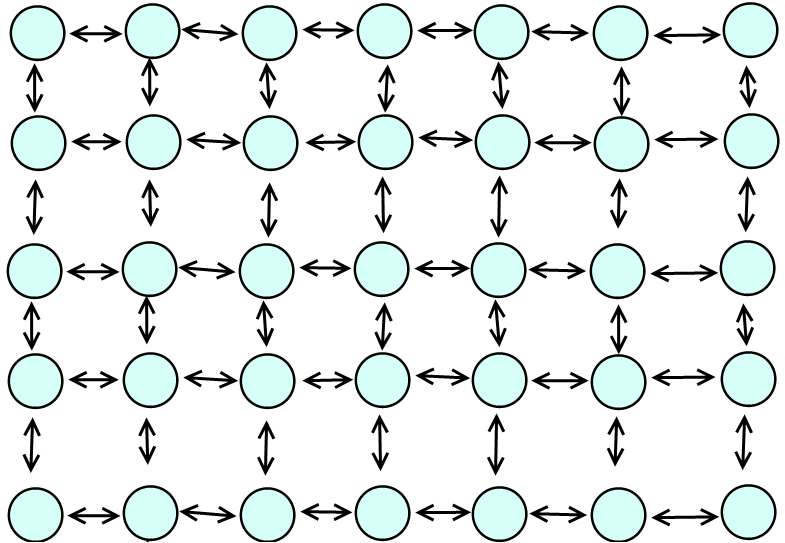
\includegraphics[width=0.5\textwidth]{Edge-connected-2D-Lattice}
\caption{Lattice Maze Space of size 7 by 5. Edges $\sim 2*size^{2}$, where the Lattice has $size^{2}$ vertices. All Lattice spaces used in this project are squares where size equals the length of both of their sides.}
\label{fig:Lattice}
\end{figure}

\begin{figure}[h]
\centering
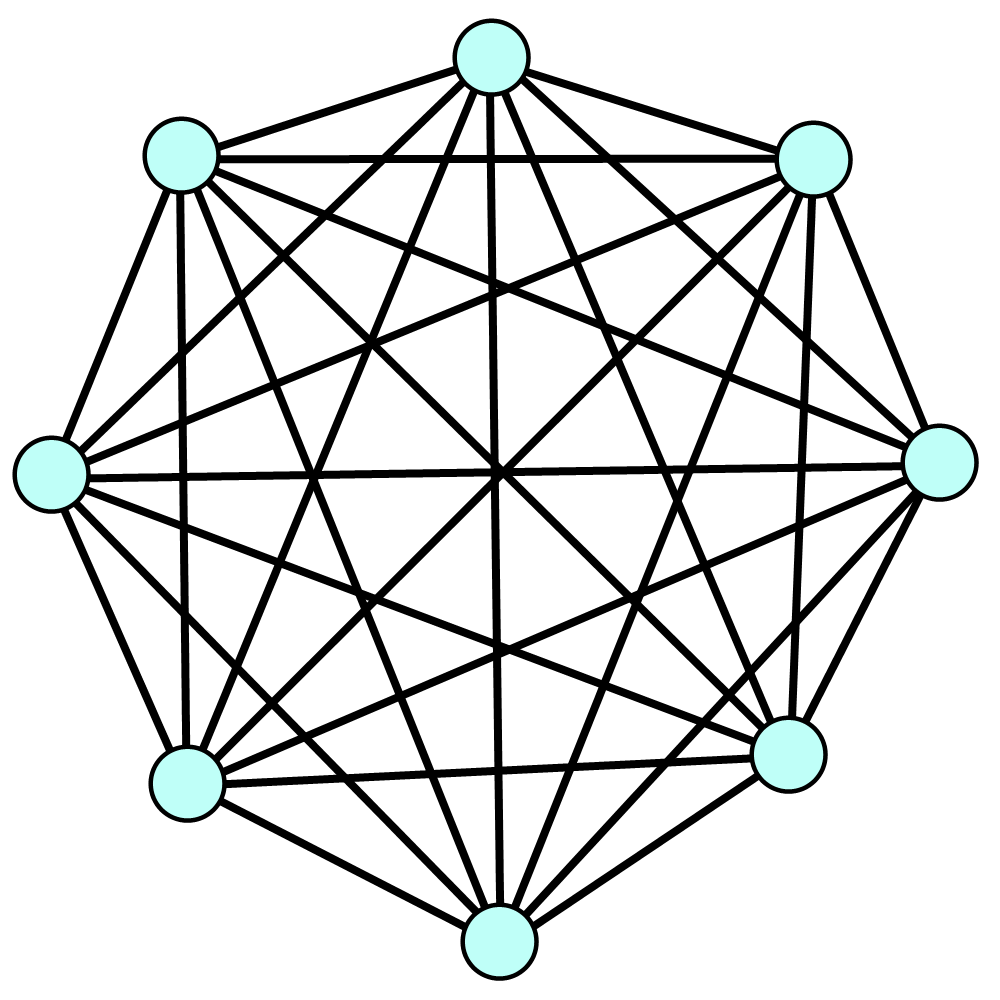
\includegraphics[width=0.5\textwidth]{K8}
\caption{Dense Maze Space of size 8. Edges $\sim size^{2}$}
\label{fig:Dense}
\end{figure}


\begin{figure}[h]
\centering
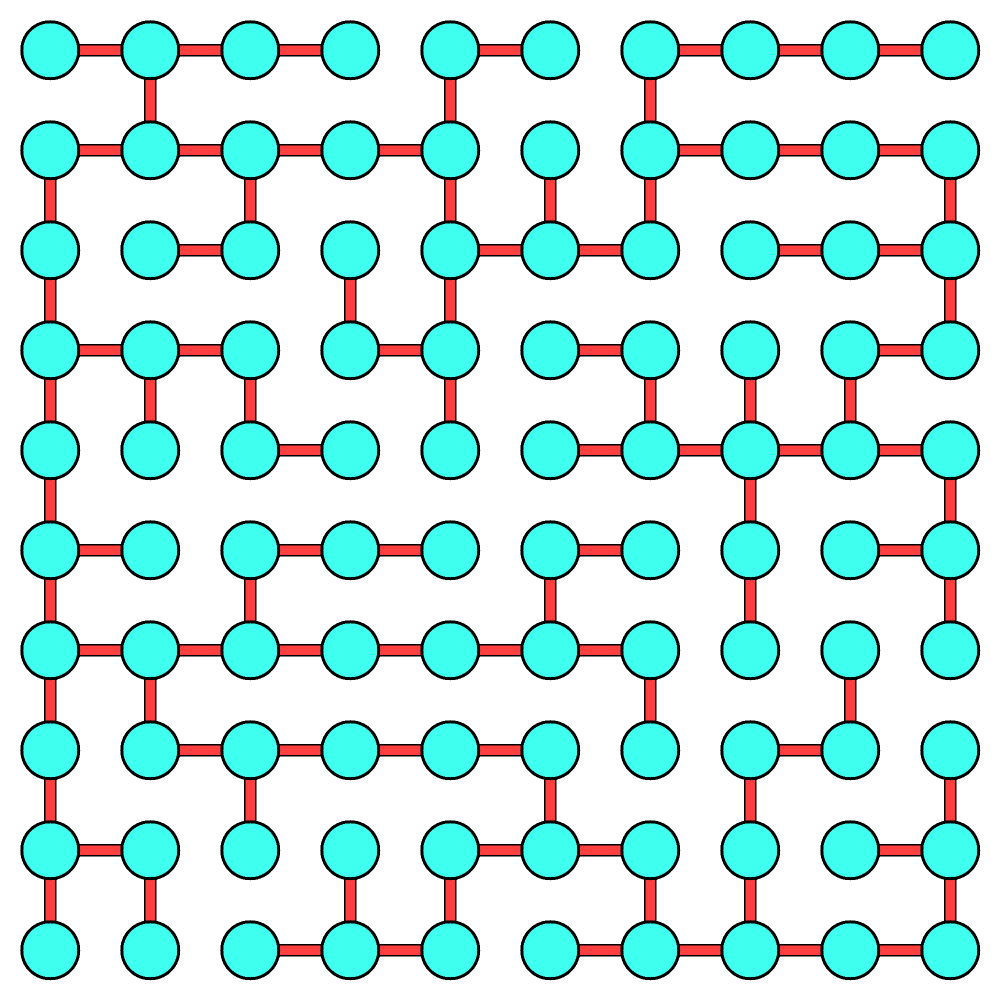
\includegraphics[width=0.5\textwidth]{Lattice1}
\caption{Example Lattice Maze result generated by our system.}
\label{fig:Lattice-result}
\end{figure}

\begin{figure}[h]
\centering
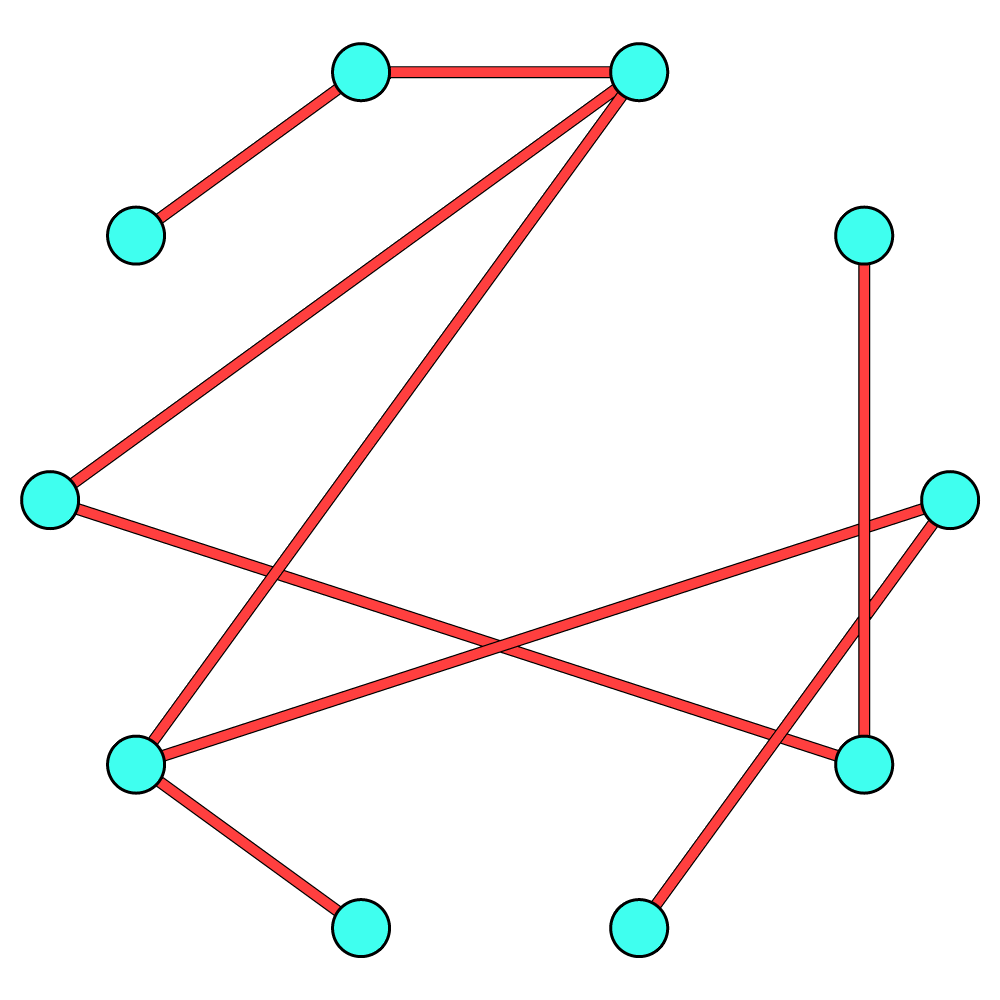
\includegraphics[width=0.5\textwidth]{Dense2}
\caption{Example Dense Maze result generated by our system.}
\label{fig:Dense-result}
\end{figure}




\begin{figure}[h]
\centering
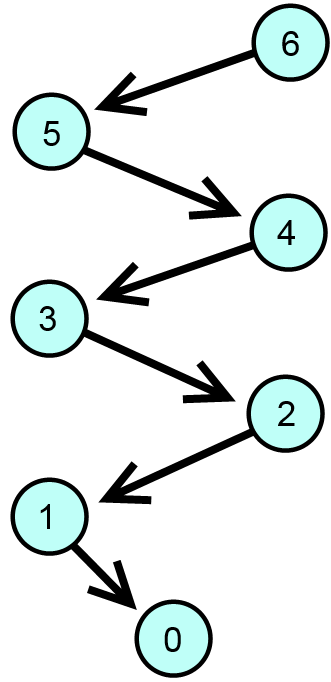
\includegraphics[width=0.25\textwidth]{UncompressedPath}
\caption{Uncompressed path of length 6.}
\label{fig:Path-NPC}
\end{figure}

\begin{figure}[h]
\centering
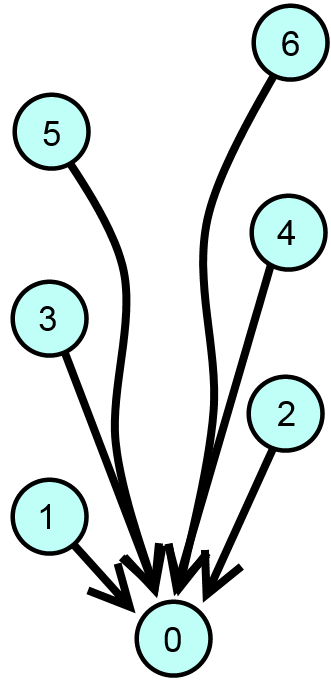
\includegraphics[width=0.25\textwidth]{FullPathCompression}
\caption{Structure after Figure \ref{fig:Path-NPC} has been fully path compressed after a find at node 6.}
\label{fig:Path-FPC}
\end{figure}

\begin{figure}[h]
\centering
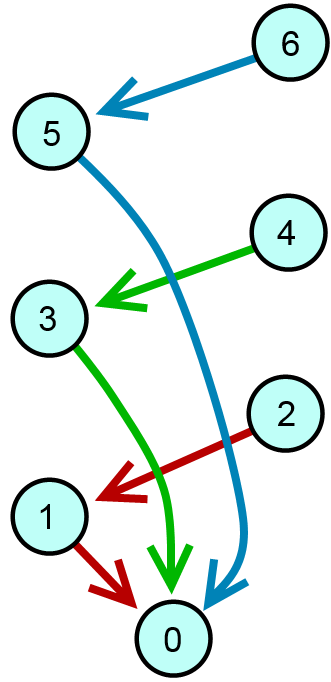
\includegraphics[width=0.25\textwidth]{ContstrainedPathCompression-k2}
\caption{Structure after Figure \ref{fig:Path-NPC} has been constrained path compressed with k = 2 after a find at node 6.}
\label{fig:Path-CPC-k2}
\end{figure}

\begin{figure}[h]
\centering
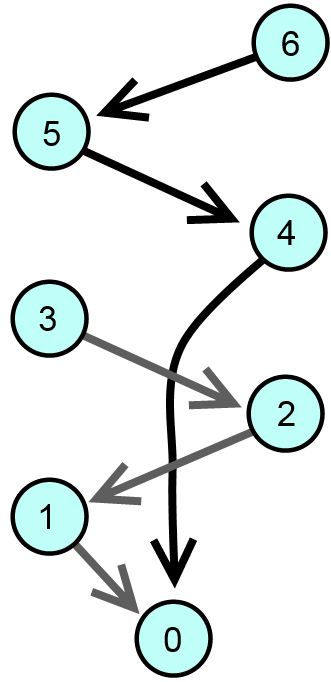
\includegraphics[width=0.25\textwidth]{ContstrainedPathCompression-k3}
\caption{Structure after Figure \ref{fig:Path-NPC} has been constrained path compressed with k = 3 after a find at node 6.}
\label{fig:Path-CPC-k3}
\end{figure}


\begin{figure}[h]
\centering
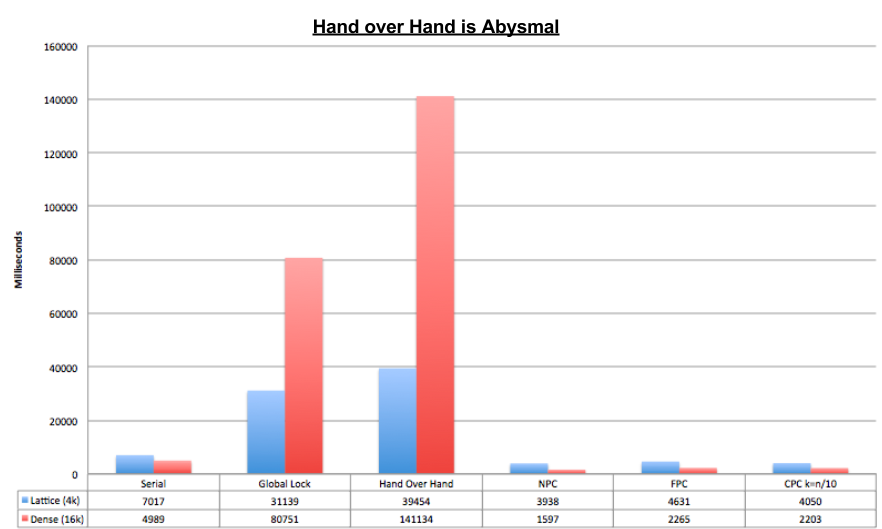
\includegraphics[width=\textwidth]{Results-Locking}
\caption{Implementations using locks behaved abysmally, most likely due to the the convergence of the operations over time. In other words, at the end of the algorithm every union find operation goes to the same root node and the locking implementations need to take and release locks prolifically so as to prevent dead lock.}
\label{fig:Results-bad-locking}
\end{figure}


\begin{figure}[h]
\centering
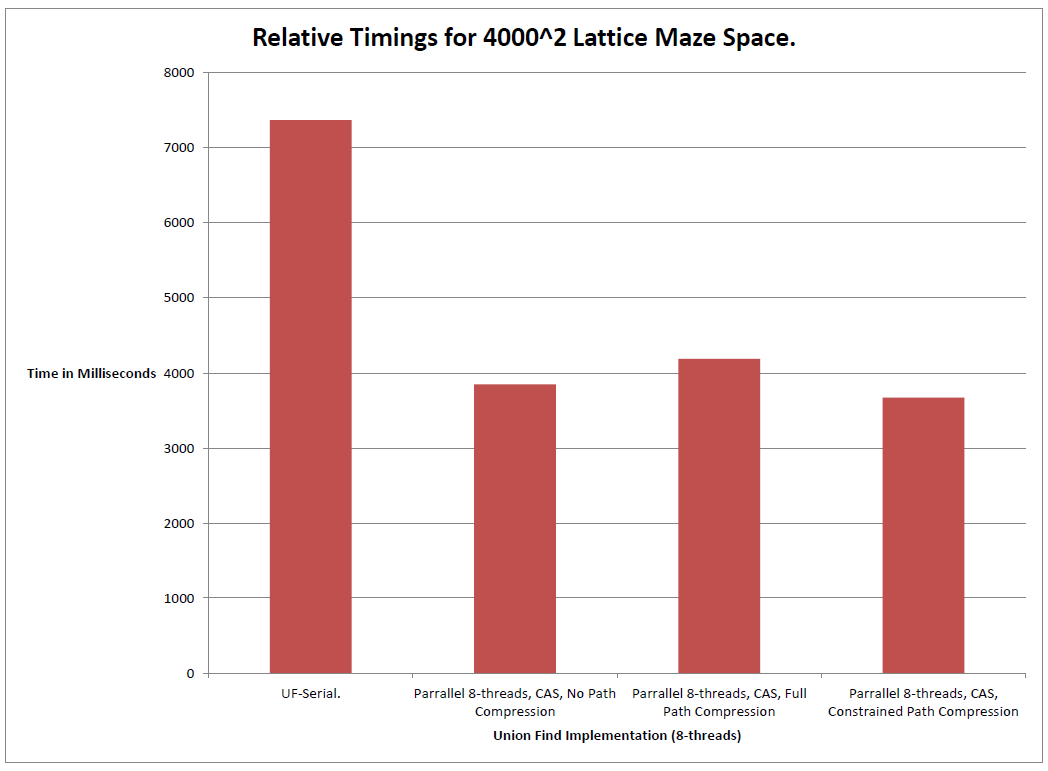
\includegraphics[width=\textwidth]{LockFreeTimings}
\caption{Lock Free Implementations consistently achieve a speedup of around 2x for the critical loop of the algorithm when run on 8 threads.}
\label{fig:Results-Lock-Free-Canonical}
\end{figure}


\begin{figure}[h]
\centering
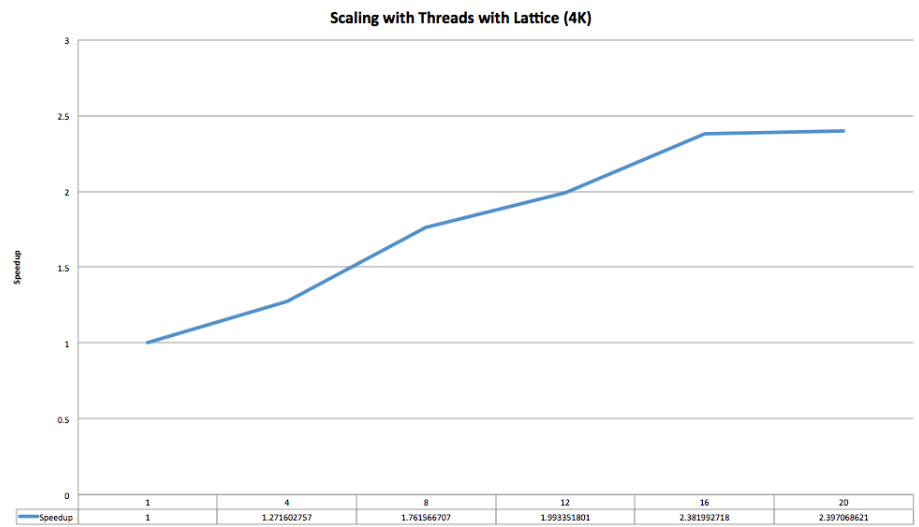
\includegraphics[width=\textwidth]{PerformanceScaling}
\caption{Lock-Free performance scales with higher thread counts for $4000$ by $4000$ lattices.}
\label{fig:Results-Scaling}
\end{figure}



\end{document}
